\subsection*{Assignment 3.a \hrule}
\textbf{Question}
\begin{quote}
Download the provided file. Each file contains haloes in a certain mass bin with variable numbers of satellites. Write down the log-likelihood corresponding to a set of random realizations of the satellite profile with some unknown $\langle N_{sat} \rangle$. Retain only the terms with a (residual) dependence on a, b and/or c (including A = A(a, b, c)). 

Find the a, b and c that maximize this likelihood. Do this separately for each different file/mass
bin. Output these values.
\end{quote}

\textbf{Solution}
\begin{quote}
Recall that the number of satellites predicted by the model on an infinite thin spherical shell at a distance x is given by,

\begin{equation}
N(x) = 4\pi A \langle N_{sat} \rangle b^{2} \left(\frac{x}{b} \right)^{a-1} \exp \left[-\left(\frac{x}{b} \right)^c \right]
\label{eq:N}
\end{equation}

here $\langle N_{sat} \rangle$ is the total amount of satellites in the halo and $A$ is a normalization constant such that the integral from $x = 0$ to $x = x_{max}$ of $N(x)$ is $\langle N_{sat} \rangle$.

In exercise 2.g it was found that the number of satellites on a sphere shell at distance $x$ is approximately distributed according to a Poisson distribution around N(x). If we assume that the distribution of satellites for haloes in the same mass bin is similar, then the probability to find the data in one of the files given the model is given by,
\begin{equation}
P(\text{data}|\text{model}) = \prod_{i=0}^{N-1} \frac{N(x_i | a, b, c)^{y_i} e^{-N(x_i | a, b, c)}}{y_i!}
\end{equation}

here $x_i$ is the distance to a satellite, $y_i$ is the number of satellites at this distance.  The optimal value's of $a$, $b$ and $c$ that maximize this probability can be found minimizing the negative log-likelihood,
\begin{equation}
- \ln(P(\text{data}|\text{model})) = -\sum_{i = 0}^{N-1} \left[ y_i \ln(N(x_i | a, b, c)) -N(x_i | a, b, c) - \ln(y_i!) \right]
\label{eq:non_assum}
\end{equation}

The satellites in the haloes of the same mass bin are, as mentioned before, expected to have the same distribution. The data of the haloes of a single file is therefore combined to create a super halo.  It is next assume that in the super halo has an infinite amount of bins.  In this case $y_i$ is either 0 or 1 and the negative log-likelihood then becomes,
\begin{equation}
- \ln(P(\text{data}|\text{model})) \approx \sum_{i=0}^{M-1} \left[- \ln(N(x_i | a, b, c)) \right] + \int_0^{x_{max}} N(x | a, b, c) dx
\end{equation}

here the sum is taken over the $M$ positions of the  satellites in the super halo. The integral over all radii is however equal to the total number of satellites in the super halo and the function to minimize therefore becomes,

\begin{equation}
- \ln(P(\text{data}|\text{model})) \approx \sum_{i=0}^{M-1} \left[- \ln(N(x_i | a, b, c)) \right] +\langle N_{sat} \rangle
\end{equation}


This function is minimized with the help of the downhill simplex method. The function is minimized withing a bounded interval: $1.1 \leq a \leq 2.5$, $0.5 \leq b \leq 2$, $1.5 \leq c \leq 4.0$. The value of $x_{max}$ is furthermore chosen to be 5. These choices make it possible to use the interpolator of the previous question to determine the value of the normalization constant $A(a, b, c)$. The value of $\langle N_{sat} \rangle$ is for each super halo set to the total amount of satellites in the super halo. The log likelihood function is finally slightly modified to prevent any minimization algorithm from walking outside the bounces. If a minimization algorithm tries an parameter that is outside one of the bounces, then the parameter will be set to the value of the bounce before evaluating the log likelihood (i.e if the downhill simplex method  tries $a = 0.47$ then $a$ is first set to 0.5 before evaluating the log likelihood).



The code that finds the optimum values of $a$, $b$ and $c$ is located in 3 files:
\textsf{./mathlib/code/assignment3.a.py},  \textsf{./mathlib/code/minimise.py}, \textsf{./mathlib/code.interpolate.py}. The first file finds the optimal values of $a$, $b$ and $c$ for each mass bin. The second file contains the implementation of the downhill simplex method. The last file contains the code for the interpolator. The produced output of the code and the code in the first two files can be found below. The code for the last file can be found in the previous assignment. 

\end{quote}


\textbf{Code - output}
\begin{quote}
\lstinputlisting{./code/assignment3_a.py}
\end{quote}

\textbf{Code - downhill}
\begin{quote}
\lstinputlisting{./code/mathlib/minimize.py}
\end{quote}

\textbf{Output - text}
\begin{quote}
The optimal values found by \textsf{./mathlib/code/assignment3.a.py}:
\lstinputlisting{./output/assignment3_a_out.txt}
\end{quote}

\textbf{Output - plots}
\begin{quote}
The fit of equation 13 to the data in the different files for the found optimal values. 

\begin{figure}[!h]
\centering
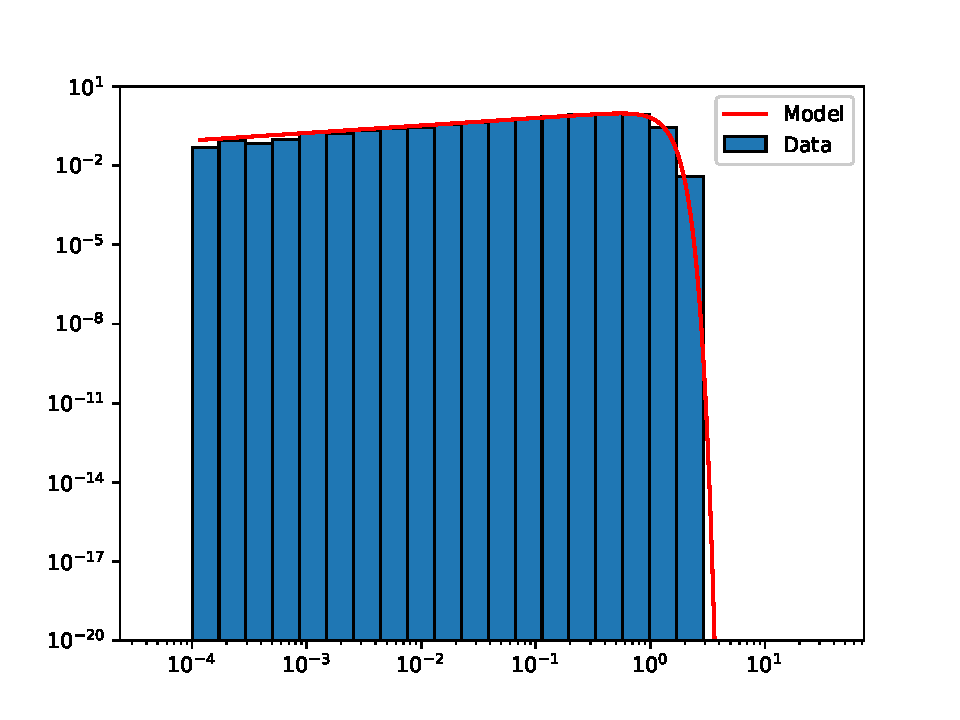
\includegraphics[scale=0.7]{plots/satgals_m11.pdf}
\caption{The model (equation 13) with the found parameters of $a$, $b$ and $c$ fitted to the data for the mass bin of $10^{11}$ $M_{\odot}$.}

\end{figure}
\newpage

\begin{figure}[!h]
\centering
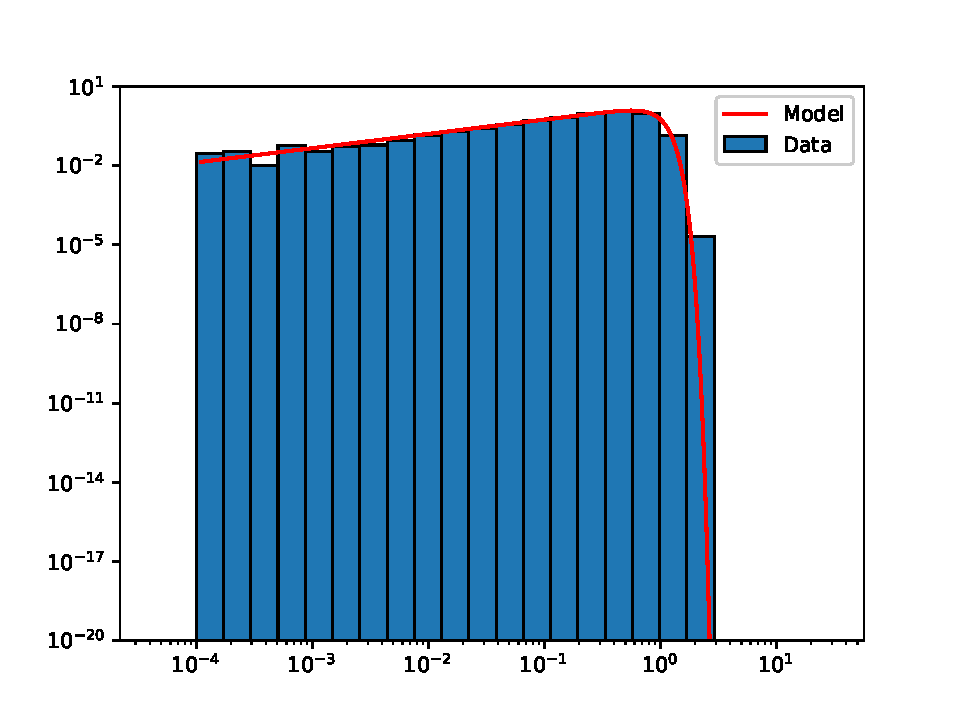
\includegraphics[scale=0.7]{plots/satgals_m12.pdf}
\caption{The model (equation 13) with the found parameters of $a$, $b$ and $c$ fitted to the data for the mass bin of $10^{12}$ $M_{\odot}$.}

\end{figure}

\begin{figure}[!ht]
\centering
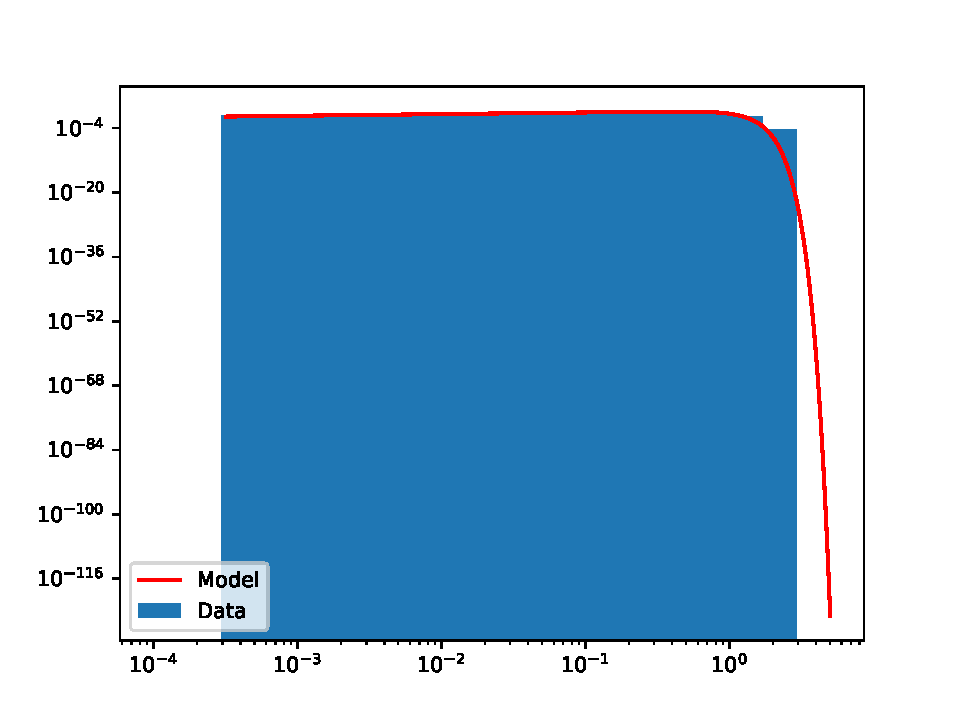
\includegraphics[scale=0.7]{plots/satgals_m13.pdf}
\caption{The model (equation 13) with the found parameters of $a$, $b$ and $c$ fitted to the data for the mass bin of $10^{13}$ $M_{\odot}$.}
\end{figure}
\newpage
\begin{figure}[!hb]
\centering
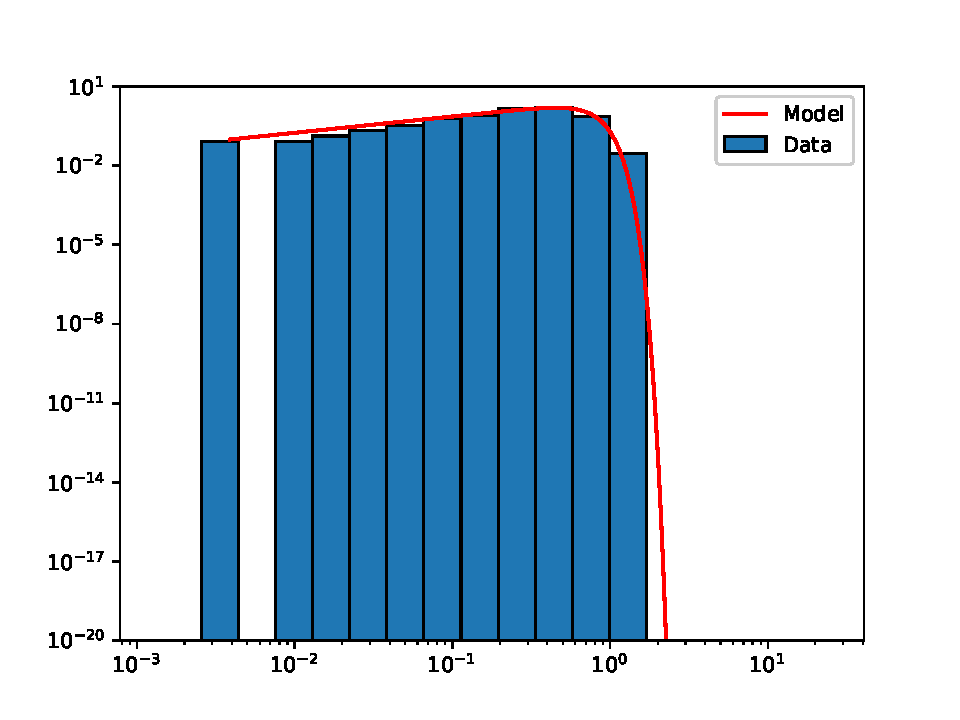
\includegraphics[scale=0.7]{plots/satgals_m14.pdf}
\caption{The model (equation 13) with the found parameters of $a$, $b$ and $c$ fitted to the data for the mass bin of $10^{14}$ $M_{\odot}$.}
\end{figure}


\begin{figure}[!ht]
\centering
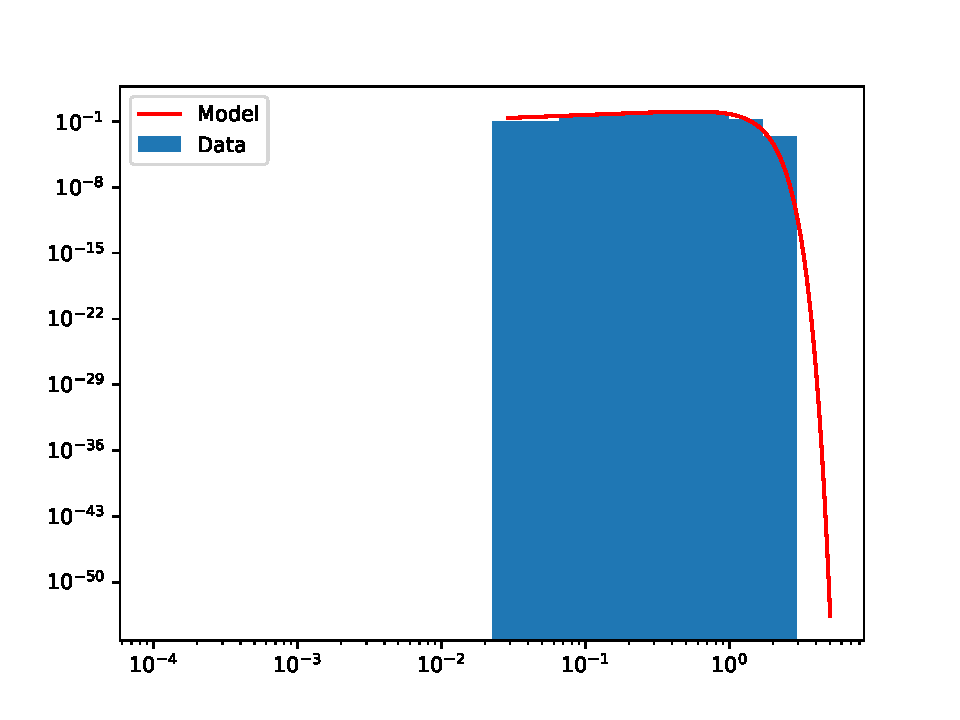
\includegraphics[scale=0.7]{plots/satgals_m15.pdf}
\caption{The model (equation 13) with the found parameters of $a$, $b$ and $c$ fitted to the data for the mass bin of $10^{15}$ $M_{\odot}$.}
\end{figure}
\end{quote}
\newpage


















